\documentclass[oneside,a4paper,14pt]{extarticle}
\usepackage[a4paper,letterpaper,top=20mm,bottom=20mm,left=20mm,right=10mm]{geometry}
\usepackage[russian]{babel}
\usepackage{indentfirst}
\usepackage{amsmath}
\usepackage{amsfonts}
\usepackage{amsthm}
\usepackage{graphicx}
\usepackage{caption}
\usepackage{titlesec}
\usepackage{minted, fancyvrb}

\titleformat{\section} {\normalsize\bfseries} {\thesection} {1em} {}
\titleformat{\subsection} {\normalsize\bfseries} {\thesubsection} {1em} {}
\titleformat{\subsubsection} {\normalsize\bfseries} {\thesubsection} {1em} {}
\renewcommand\baselinestretch{1.45}\normalsize
\setlength{\parindent}{1.25cm}

\begin{document}

\newpage
\thispagestyle{empty}
\begin{center}
	МИНИСТЕРСТВО НАУКИ И ВЫСШЕГО ОБРАЗОВАНИЯ РОССИЙСКОЙ ФЕДЕРАЦИИ ФЕДЕРАЛЬНОЕ ГОСУДАРСТВЕННОЕ БЮДЖЕТНОЕ ОБРАЗОВАТЕЛЬНОЕ УЧРЕЖДЕНИЕ ВЫСШЕГО ОБРАЗОВАНИЯ\\
	«ВЯТСКИЙ ГОСУДАРСТВЕННЫЙ УНИВЕРСИТЕТ»\\
	Институт математики и информационных систем\\
	Факультет автоматики и вычислительной техники\\
	Кафедра электронных вычислительных машин
\end{center}
\vspace{10mm}

\hfill
\begin{tabular}{l}
  \footnotesize Дата сдачи на проверку: \\
  \footnotesize <<\rule[-1mm]{5mm}{0.10mm}\/>>\rule[-1mm]{20mm}{0.10mm}\ 2025 г.\\
  \footnotesize Проверено: \\
  \footnotesize <<\rule[-1mm]{5mm}{0.10mm}\/>>\rule[-1mm]{20mm}{0.10mm}\ 2025 г. \\
\end{tabular}
\vfill

\begin{center}
  ГРАФЫ. ОПЕРАЦИИ НАД ГРАФАМИ.\\
	Отчёт по лабораторной работе №4\\
	по дисциплине\\
	<<Дискретная математика>>\\
\end{center}
\vspace{25mm}
\noindent
\begin{tabular}{ll}
	Разработал студент гр. ИВТб-1301-05-00 & \rule[-1mm]{30mm}{0.10mm}\,/Черкасов А. А./   \\
	                                       & \hspace{8mm}\footnotesize(подпись)            \\
	Проверила преподаватель                & \rule[-1mm]{30mm}{0.10mm}\,/Пахарева И. В./ \\
	                                       & \hspace{8mm}\footnotesize(подпись)            \\
\end{tabular}

\noindent
  \begin{tabular}{lp{58mm}r}
    Работа защищена &  & <<\rule[-1mm]{5mm}{0.10mm}\/>>\rule[-1mm]{30mm}{0.10mm}\ 2025 г.
  \end{tabular}
  \vfill

\begin{center}
	Киров\\
	2025
\end{center}

\newpage\thispagestyle{plain}

\section*{Цель}

Цель работы: Изучить операцию построения дополнения для неориентированного графа на основе представления в виде матрицы смежности и разработать программу, которая по заданной в файле input.txt матрице смежности формирует матрицу смежности дополненного графа. Это позволяет закрепить навыки работы с представлением графов в памяти компьютера и понять принципы формирования нового графа на основании исходного.

\section*{Задание}
\begin{itemize}
	\item[$-$] Неориентированный граф G1 задается матрицей смежности, которая записана в файле \texttt{input.txt}. Размерность графа задается в программе (вершин $\geq 5$, дуг $\geq 7$)
	\item[$-$] Сформировать дополнение графа.
\end{itemize}
\section*{Решение}

Схема алгоритма решения представлена на рисунке 1.1 и 1.2. Примеры работы программы представлены на рисунках 2.1 и 2.4, графы построенные по матрицам из примеров представлены на рисунках 2.2, 2.3, 2.5, 2.6. Исходный код решения представлен в Приложении A1.

\clearpage
\begin{figure}[H]
	\centering
	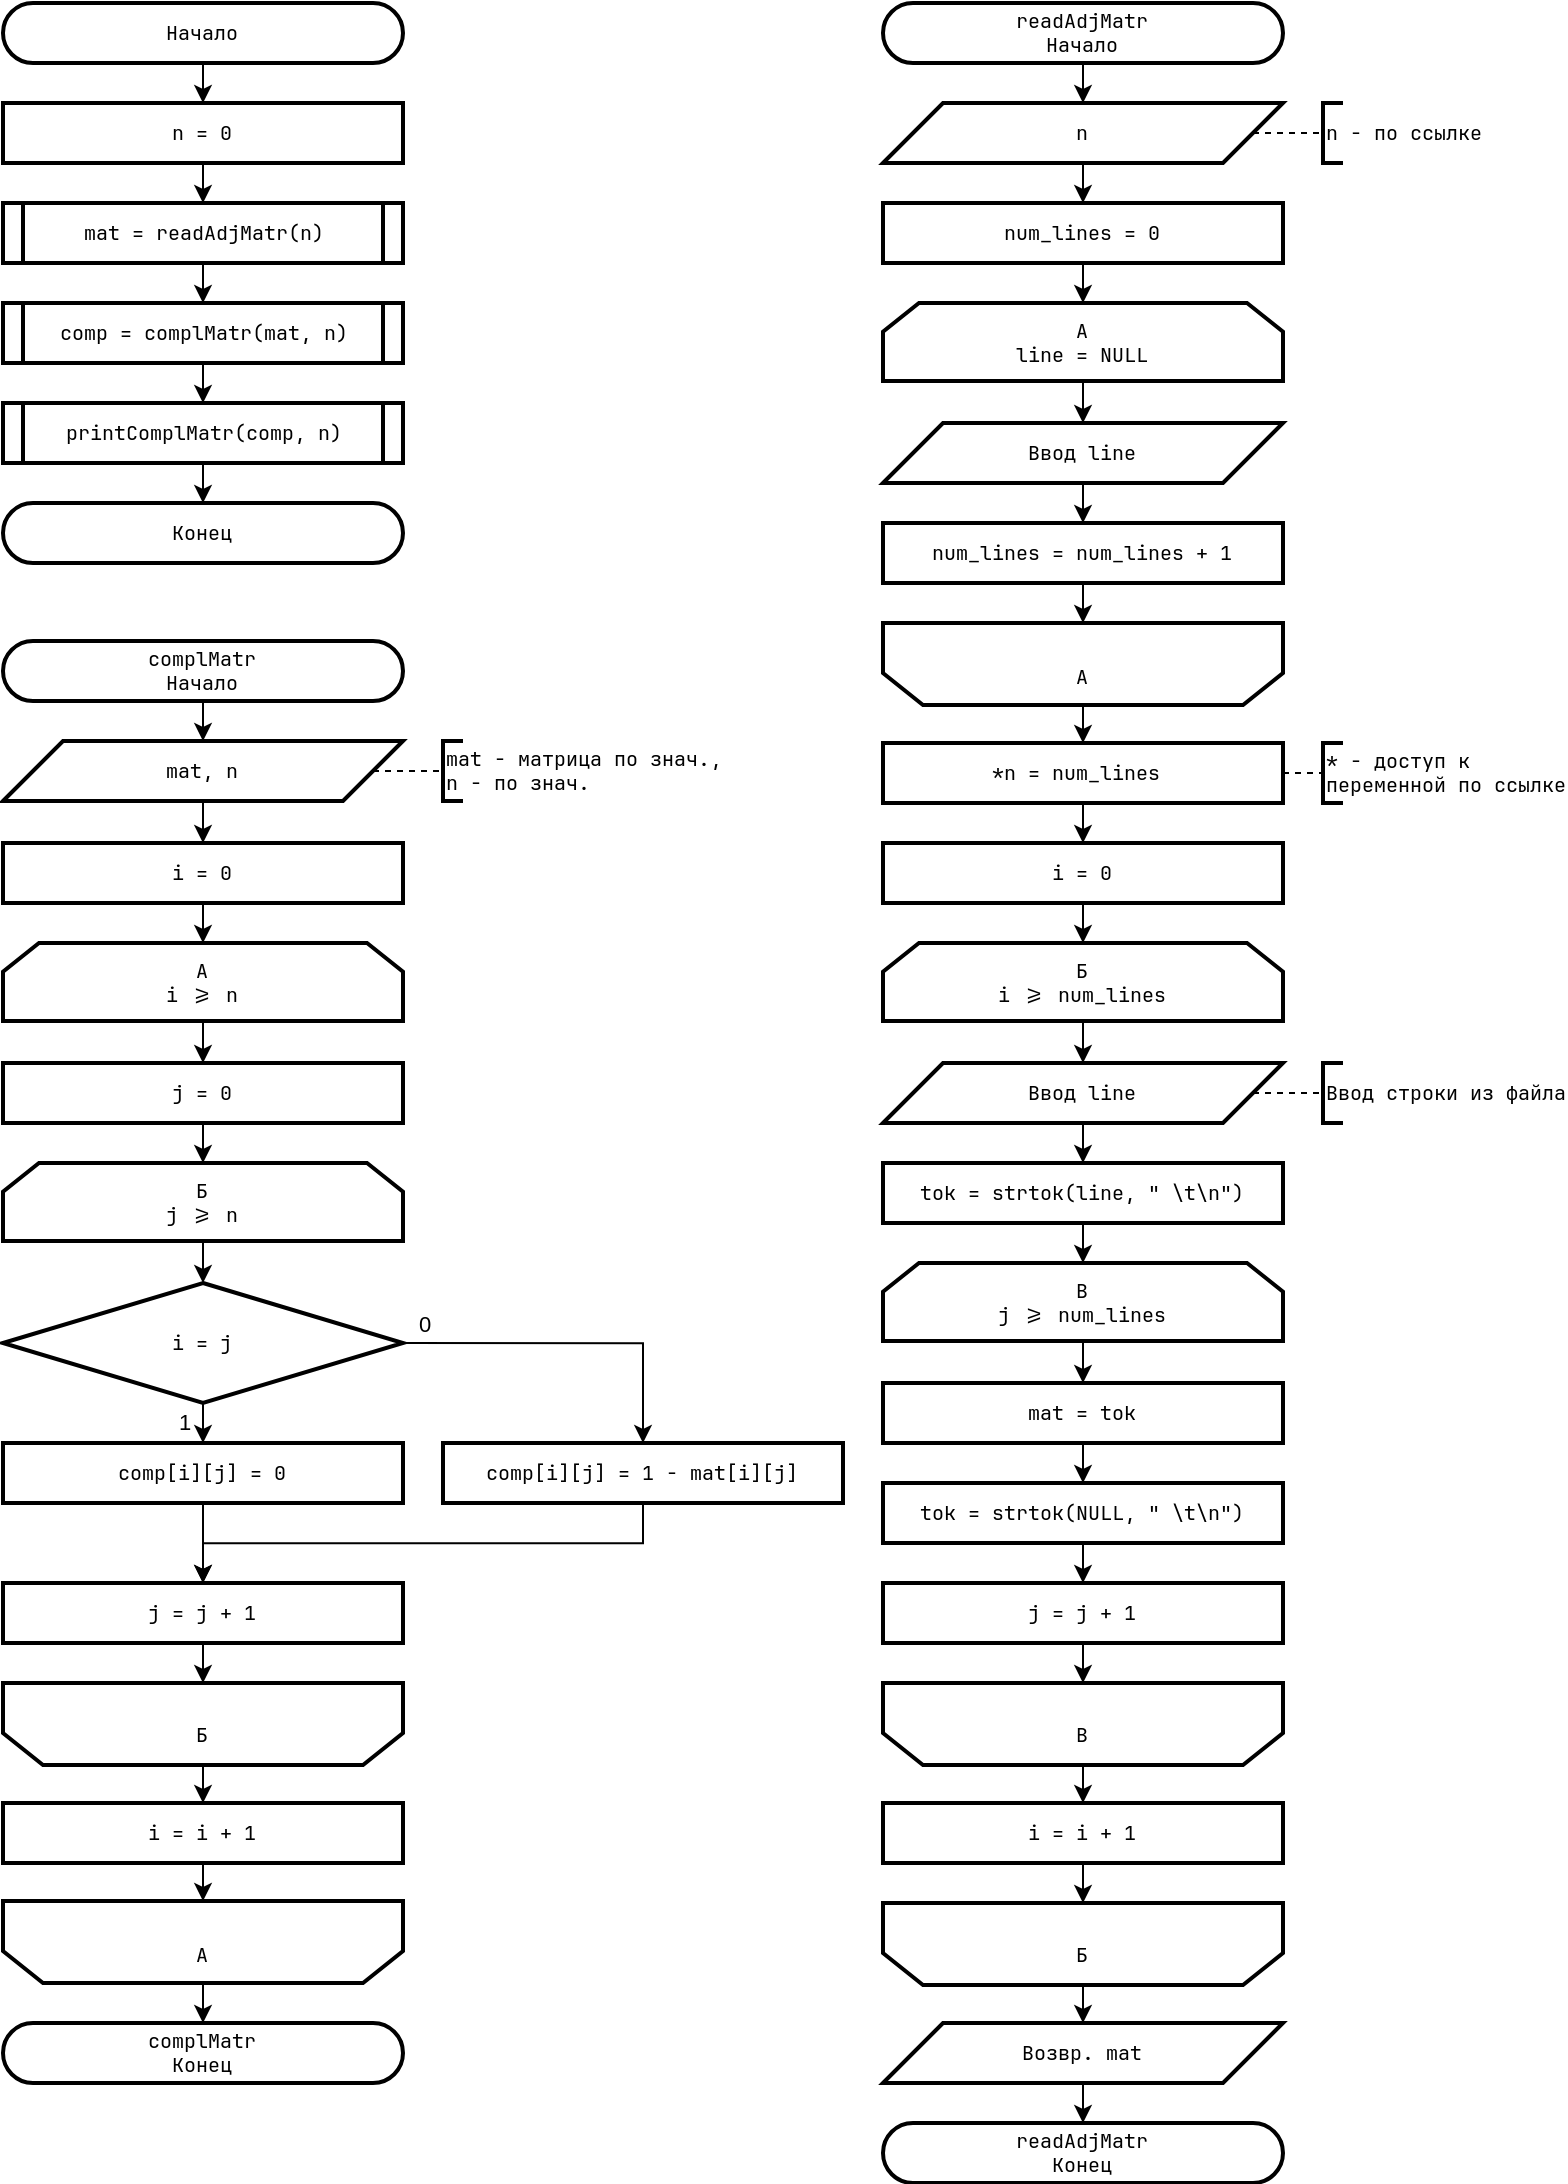
\includegraphics[height=0.9\textheight]{pics/flowchart1.png}
	\caption*{Рисунок 1.1 - Схема алгоритма основной программы, подпрограммы чтения матрицы из файла, подпрограмма формирования дополненной матрицы.}
\end{figure}

\clearpage
\begin{figure}[H]
	\centering
	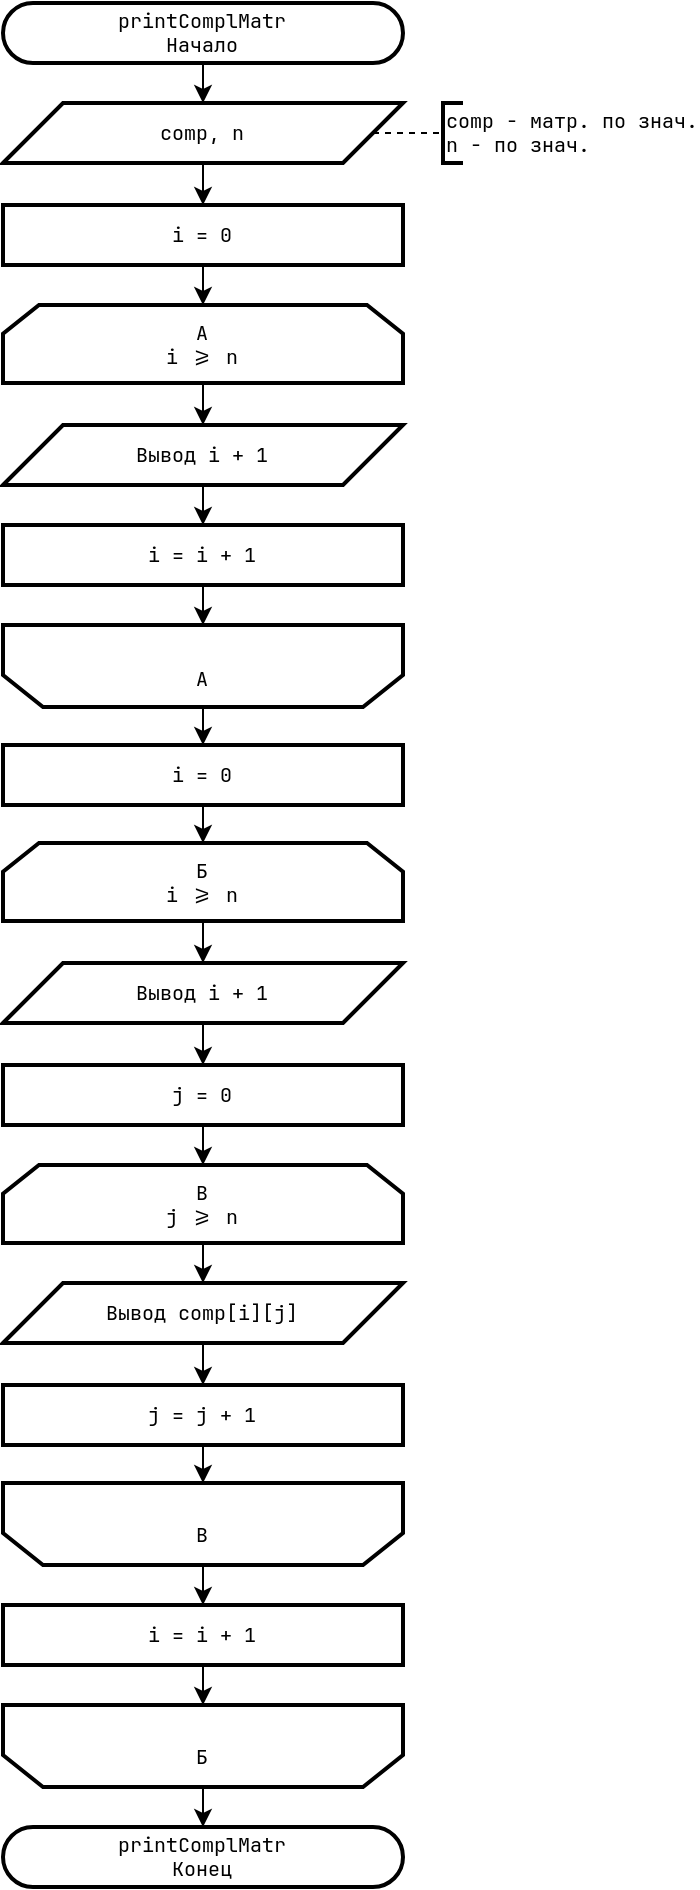
\includegraphics[height=0.9\textheight]{pics/flowchart2.png}
	\caption*{Рисунок 1.1 - Схема алгоритма подпрограммы вывода итоговой матрицы.}
\end{figure}

\clearpage
\begin{figure}[H]
	\centering
	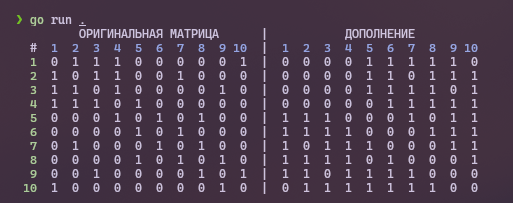
\includegraphics[width=0.9\textwidth]{pics/screen1.png}
	\caption*{Рисунок 2.1 - Пример работы программы 1.}
\end{figure}

\begin{figure}[H]
	\centering
	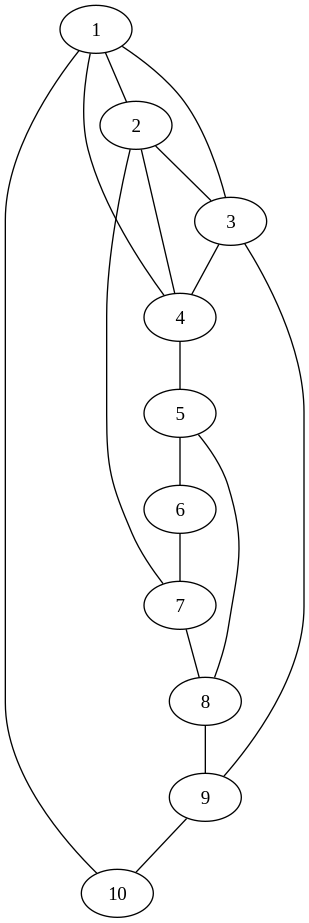
\includegraphics[height=0.5\textheight]{pics/original_graph1.png}
	\caption*{Рисунок 2.2 - Оригинальный граф построенный по входной матрице 1 примера.}
\end{figure}

\begin{figure}[H]
	\centering
	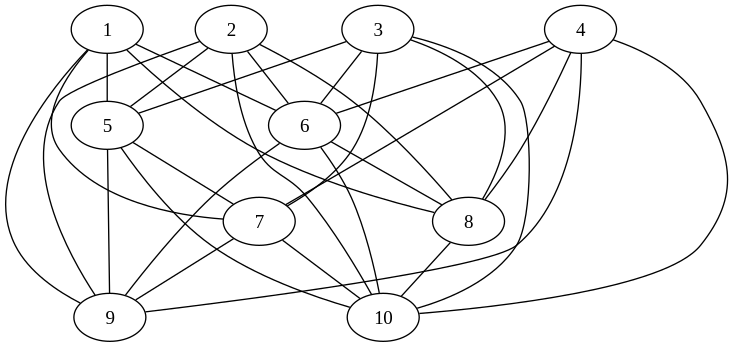
\includegraphics[width=0.9\textwidth]{pics/complement_graph1.png}
	\caption*{Рисунок 2.3 - Дополненный граф построенный по итоговой матрице 1 примера.}
\end{figure}

\clearpage
\begin{figure}[H]
	\centering
	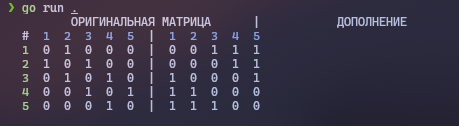
\includegraphics[width=0.9\textwidth]{pics/screen2.png}
	\caption*{Рисунок 2.4 - Пример работы программы 2.}
\end{figure}

\begin{figure}[H]
	\centering
	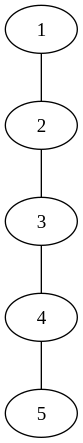
\includegraphics[height=0.25\textheight]{pics/original_graph2.png}
	\caption*{Рисунок 2.5 - Оригинальный граф построенный по входной матрице 2 примера.}
\end{figure}

\begin{figure}[H]
	\centering
	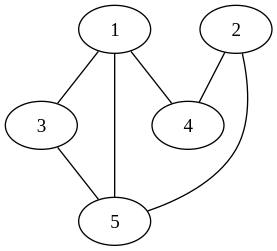
\includegraphics[width=0.3\textwidth]{pics/complement_graph2.png}
	\caption*{Рисунок 2.6 - Дополненный граф построенный по итоговой матрице 2 примера.}
\end{figure}

\section*{Вывод}

В ходе выполнения лабораторной работы были изучены основы представления неориентированных графов с помощью матрицы смежности, а также алгоритм построения дополнения графа. Реализованная программа на языке Go, которая осуществляет чтение исходной матрицы из файла, проверяет её корректность, формирует матрицу дополненного графа и выводит результат. Работа позволила закрепить навыки работы с графами,
улучшить понимание операций над графами и применение их в программировании.


\setminted{style = rainbow_dash, fontsize = \small} % https://pygments.org/styles/

\newpage
\section*{Приложение А1. Исходный код}
\inputminted{go}{code/main.go}

\end{document}
